% Generated by Claude Opus 5 (Anthropic) — panels from postprocess/paper_fig_model.py
% Real data: (a),(b) Autoware session fish_20260906_151532; (c),(d) Isaac ROS unet session fish_20260830_224846.
\begin{figure*}[t]\centering
  \begin{subfigure}[t]{0.49\textwidth}\centering
    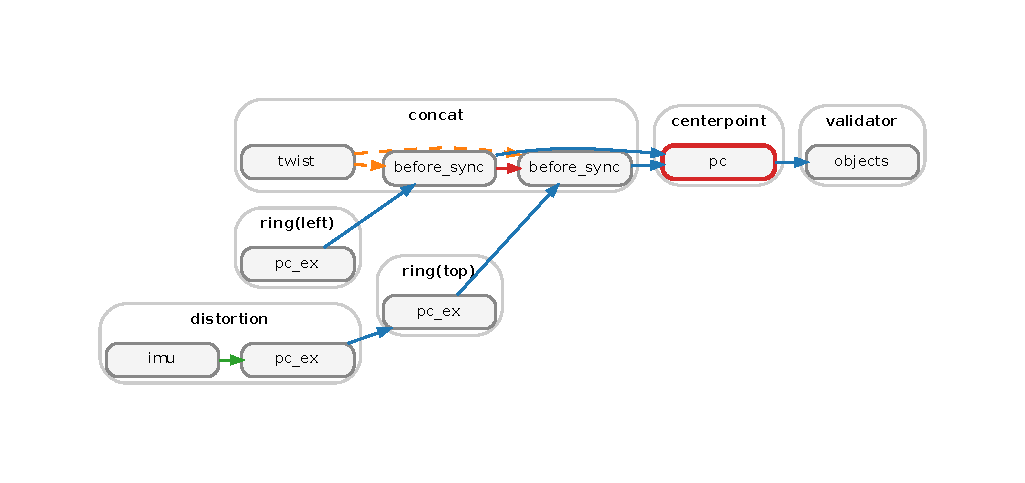
\includegraphics[width=\linewidth]{figures/model/panel_a}
    \caption{callback layer: message, join, state and polled edges; the GPU submitter is outlined in red}
  \end{subfigure}\hfill
  \begin{subfigure}[t]{0.49\textwidth}\centering
    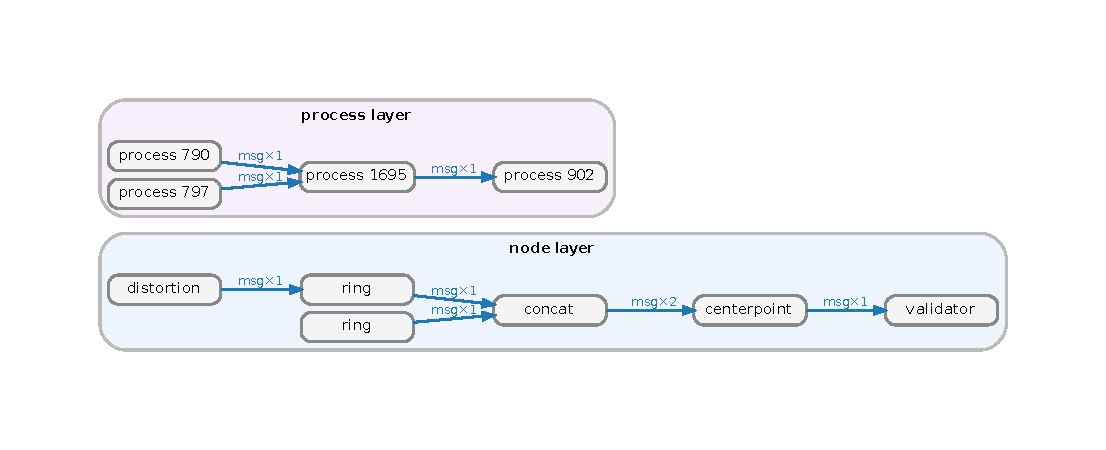
\includegraphics[width=\linewidth]{figures/model/panel_b}
    \caption{the same fragment lifted to the node and the process layer; each edge is the set it aggregates}
  \end{subfigure}

  \vspace{2pt}
  \begin{subfigure}[t]{0.49\textwidth}\centering
    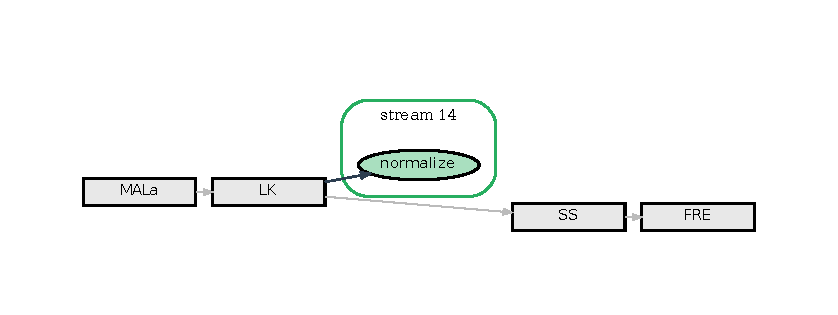
\includegraphics[width=\linewidth]{figures/model/panel_c}
    \caption{typed DAG of one invocation: CPU calls, kernels on the SMs, transfers on the copy engines}
  \end{subfigure}\hfill
  \begin{subfigure}[t]{0.49\textwidth}\centering
    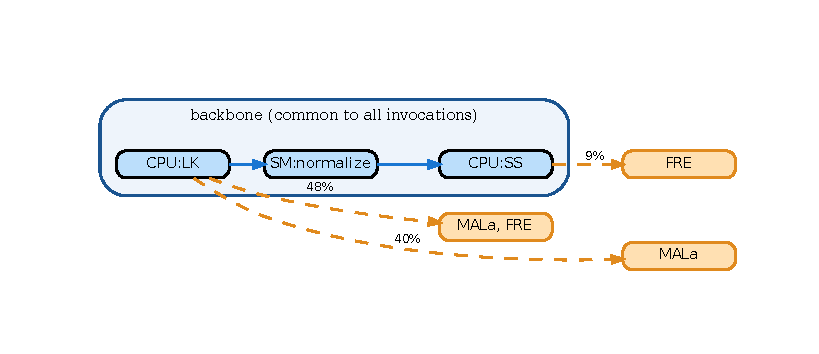
\includegraphics[width=\linewidth]{figures/model/panel_d}
    \caption{conditional graph of the same callback: backbone common to all invocations plus branches}
  \end{subfigure}
  \caption{What FISH extracts from an unmodified stack. (a),(b) Autoware:
    the lidar pipeline from the per-lidar filters to the CenterPoint detector,
    with the join of the concatenation node, the sample-and-hold reads of the
    distortion corrector and the concatenation node, and the same fragment
    after lifting. (c),(d) Isaac ROS: one NITROS callback, 29\,335 invocations,
    nine distinct GPU shapes.}
  \label{fig:model}
\end{figure*}
